\input{sol_pre.tex}
\input{q_2026-10-03_2.tex}
\begin{document}
\input{sol_head.tex}

%================= 1
\Savol{1}
$255255=255\cdot1001=(3\cdot5\cdot17)\cdot(7\cdot11\cdot13)$ — 6 ta turli tub köpaytuvçi, har biri birinçi darajada.
\[\tau=(1+1)^6=64.\]
\Javob{B) 64}

%================= 2
\Savol{2}
1) $\sqrt[3]{2-\sqrt5}$ — toq darajali ildiz, manfiy sondan ham mavjud: haqiqiy. \ 2) $\sqrt{-144}$ — haqiqiy emas. \ 3) $-\sqrt{64}=-8$ — haqiqiy.\\
4) $\sqrt{157}<\sqrt{169}=13$, ya'ni $\sqrt{157}-13<0$ — haqiqiy emas. \ 5) $3{,}8(6)$ — haqiqiy.\\
Jami 3 ta.
\Javob{B) 3 ta}

%================= 3
\Savol{3}
Yaqinlaşiş tezligi $350-320=30$ m/min. \quad $t=\dfrac{120}{30}=4$ min.
\Javob{A) 4}

%================= 4
\Savol{4}
Töğri işlaganlar uluşi $100\%-12\%-32\%=56\%$. \quad $0{,}56\cdot N=14\Rightarrow N=25$.
\Javob{A) 25}

%================= 5
\Savol{5}
\[2^{-26}\cdot2^{-24}\cdot2^{-15}\cdot2^n=2^{n-65}.\]
Natural son bölişi uçun $n-65\ge0$, eng kiçik $n=65$.
\Javob{D) 65}

%================= 6
\Savol{6}
$\left(\dfrac{3+\sqrt5}2\right)^3=\dfrac{(3+\sqrt5)^2(3+\sqrt5)}8=\dfrac{(14+6\sqrt5)(3+\sqrt5)}8=\dfrac{72+32\sqrt5}8=9+4\sqrt5$. \ Xuddi şunday $9-4\sqrt5=\left(\frac{3-\sqrt5}2\right)^3$.
\[\frac{3+\sqrt5}2+\frac{3-\sqrt5}2=3.\]
\Javob{C) 3}

%================= 7
\Savol{7}
$N=\sqrt{100+\sqrt n}+\sqrt{100-\sqrt n}$ ni kvadratga oşiramiz:
\[N^2=200+2\sqrt{10000-n}\ \Rightarrow\ \sqrt{10000-n}=\frac{N^2-200}2.\]
$n$ qança kiçik bölsa, $N$ şunça katta. $0<n\le10000$ da $200\le N^2<400$.\\
$N=19$: $\sqrt{10000-n}=80{,}5\Rightarrow n=3519{,}75$ — natural emas. \ $N=18$: $\sqrt{10000-n}=62\Rightarrow n=10000-3844=6156$.
\Javob{A) 6156}

%================= 8
\Savol{8}
$a_2+a_{10}=2a_6=20\Rightarrow a_6=a_1+5d=10$, \ $a_1=10-5d$.
\[(10-5d)(10-4d)=10\ \Rightarrow\ 20d^2-90d+90=0\ \Rightarrow\ 2d^2-9d+9=0\ \Rightarrow\ d=3\ \text{yoki}\ d=\tfrac32.\]
$a_3=a_1+2d=10-3d$: \ $d=3\Rightarrow a_3=1$; \ $d=\frac32\Rightarrow a_3=\frac{11}2$.
\Javob{C) 1 yoki $\frac{11}2$}

%================= 9
\Savol{9}
$a_1=b_1=b$, \ $a_2=b_2=bq$ $\Rightarrow$ $d=b(q-1)$.
\[a_7=b+6b(q-1)=bq^2\ \Rightarrow\ q^2-6q+5=0\ \Rightarrow\ q=5\quad(q=1\ \text{— özgarmas ketma-ketlik}).\]
\Javob{D) 5}

%================= 10
\Savol{10}
\[x^2-\tfrac1{y^2}=\tfrac{(xy-1)(xy+1)}{y^2},\quad y+\tfrac1x=\tfrac{xy+1}x,\quad y^2-\tfrac1{x^2}=\tfrac{(xy-1)(xy+1)}{x^2},\quad x-\tfrac1y=\tfrac{xy-1}y.\]
Surat: $\dfrac{(xy-1)^x(xy+1)^x}{y^{2x}}\cdot\dfrac{(xy+1)^{y-x}}{x^{y-x}}=\dfrac{(xy-1)^x(xy+1)^y}{y^{2x}x^{y-x}}$; \quad maxraj: $\dfrac{(xy-1)^y(xy+1)^y}{x^{2y}}\cdot\dfrac{(xy-1)^{x-y}}{y^{x-y}}=\dfrac{(xy-1)^x(xy+1)^y}{x^{2y}y^{x-y}}$.
\[\frac{x^{2y}\,y^{x-y}}{y^{2x}\,x^{y-x}}=x^{x+y}\,y^{-x-y}=\left(\frac xy\right)^{x+y}.\]
\Javob{C) $\left(\frac xy\right)^{x+y}$}

%================= 11
\Savol{11}
$(x+y)^2-z^2=(x+y-z)(x+y+z)$, \quad $x^2-y^2-z^2+2yz=x^2-(y-z)^2=(x-y+z)(x+y-z)$.
\[\frac{x+y+z}{(x+y-z)(x+y+z)}\cdot(x-y+z)(x+y-z)=x-y+z.\]
\Javob{A) $x-y+z$}

%================= 12
\Savol{12}
$\left(\sqrt[3]7\right)^{\frac3{\log_27}}=7^{\frac1{\log_27}}=7^{\log_72}=2$. \quad $\log_49\cdot\log_913\cdot\log_{13}6=\log_46$.
\[2-\log_46+\log_424=2+\log_4\frac{24}6=2+1=3.\]
\Javob{C) 3}

%================= 13
\Savol{13}
\[\frac1{\sin^240^\circ}-\frac1{\cos^240^\circ}=\frac{\cos^240^\circ-\sin^240^\circ}{\sin^240^\circ\cos^240^\circ}=\frac{\cos80^\circ}{\frac14\sin^280^\circ},\qquad \frac{2\tg40^\circ}{1-\tg^240^\circ}=\tg80^\circ.\]
\[\frac{4\cos80^\circ}{\sin^280^\circ}\cdot\sin80^\circ\cdot\frac{\sin80^\circ}{\cos80^\circ}=4.\]
\Javob{A) 4}

%================= 14
\Savol{14}
$\sin\frac\pi{14}=\cos\frac{3\pi}7$. Ifoda $=\dfrac{1-4\sin\frac\pi{14}\cos\frac{2\pi}7}{\sin\frac\pi{14}}$, \ $4\sin\frac\pi{14}\cos\frac{4\pi}{14}=2\left(\sin\frac{5\pi}{14}-\sin\frac{3\pi}{14}\right)=2\left(\cos\frac\pi7-\cos\frac{2\pi}7\right)$.\\
Ma'lum ayniyat $\cos\frac\pi7-\cos\frac{2\pi}7+\cos\frac{3\pi}7=\frac12$ (uni $2\sin\frac\pi7$ ga köpaytirib tekşiriş mumkin: yiğindi $\sin\frac\pi7$ ga teng böladi). Demak
\[1-2\Bigl(\cos\tfrac\pi7-\cos\tfrac{2\pi}7\Bigr)=2\cos\tfrac{3\pi}7=2\sin\tfrac\pi{14}\ \Rightarrow\ \frac{2\sin\frac\pi{14}}{\sin\frac\pi{14}}=2.\]
\Javob{B) 2}

%================= 15
\Savol{15}
$15^x-50\cdot5^x+300-6\cdot3^x=0$. Guruhlaymiz ($15^x=5^x\cdot3^x$):
\[5^x(3^x-50)-6(3^x-50)=0\ \Rightarrow\ (5^x-6)(3^x-50)=0\ \Rightarrow\ x=\log_56,\ \ x=\log_350.\]
\Javob{B) 2 ta}

%================= 16
\Savol{16}
Aniqlaniş sohasi $[2;6]$. Ikkala tomon manfiymas, 4-darajaga oşiramiz:
\[(x-2)^2\ge6-x\ \Rightarrow\ x^2-3x-2\ge0\ \Rightarrow\ x\ge\frac{3+\sqrt{17}}2\approx3{,}56.\]
$x\in[3{,}56\ldots;6]$: butun sonlar $4;5;6$ — 3 ta.
\Javob{C) 3}

%================= 17
\Savol{17}
$x^2+11x+24=(x+3)(x+8)$, \ $x^2+9x+18=(x+3)(x+6)$. Umumiy maxrajga keltiramiz:
\[\frac{8x+43-(x+8)(x+6)}{(x+3)(x+8)(x+6)^2}=\frac{-(x^2+6x+5)}{(x+3)(x+8)(x+6)^2}\ge0\ \Rightarrow\ \frac{(x+1)(x+5)}{(x+3)(x+8)(x+6)^2}\le0.\]
Oraliqlar usuli ($x\ne-6$): \ $x\in(-8;-6)\cup(-6;-5]\cup(-3;-1]$.\\
Butun yeçimlar: $-7,\,-5,\,-2,\,-1$; \ yiğindi $-15$.
\Javob{C) $-15$}

%================= 18
\Savol{18}
$|x-1|-2=\pm2$: \ $|x-1|=4\Rightarrow x=5,\ x=-3$; \ $|x-1|=0\Rightarrow x=1$. Jami 3 ta.
\Javob{C) 3}

%================= 19
\Savol{19}
Ikki turli manfiy ildiz: $D>0$, $x_1x_2>0$, $x_1+x_2<0$.
\[D=144-12a>0\Rightarrow a<12;\qquad x_1x_2=3a>0\Rightarrow a>0;\qquad x_1+x_2=-12<0.\]
$a\in\{1,2,\dots,11\}$ — 11 ta.
\Javob{B) 11}

%================= 20
\Savol{20}
$f(2x)=4x-3$, \ $f(x-1)=2(x-1)-3=2x-5$.
\[3\bigl(4x-3-2(2x-5)\bigr)=3\cdot7=21.\]
\Javob{B) 21}

%================= 21
\Savol{21}
Nollar teng bölişi uçun $a\ne0$ (aks holda çiziqli funksiya) va $D=0$:
\[a^2x^2-12x+9:\quad D=144-36a^2=0\ \Rightarrow\ a=\pm2.\qquad 2+(-2)=0.\]
\Javob{C) 0}

%================= 22
\Savol{22}
\[f'(x)=2(x^2-2)\cdot2x+3(x^3-2)^2\cdot3x^2,\qquad f'(1)=2\cdot(-1)\cdot2+3\cdot1\cdot3=-4+9=5.\]
\Javob{D) 5}

%================= 23
\Savol{23}
$t=\sqrt[3]{2x+1}$: \ $x=\frac{t^3-1}2$, \ $dx=\frac32t^2dt$, \ $x+1=\frac{t^3+1}2$; \ $t:1\to3$.
\[\int_1^3\frac{t^3+1}{2t}\cdot\frac32t^2\,dt=\frac34\int_1^3(t^4+t)\,dt=\frac34\left(\frac{t^5}5+\frac{t^2}2\right)\Big|_1^3=\frac34\left(\frac{242}5+4\right)=\frac34\cdot\frac{262}5=39{,}3.\]
\Javob{D) 39,3}

%================= 24
\Savol{24}
\fig{\begin{tikzpicture}[scale=0.85]
\coordinate (O) at (0,0); \coordinate (B) at (90:2); \coordinate (A) at (240:2); \coordinate (C) at (290:2);
\draw[thick] (O) circle (2); \draw[thick] (A)--(B)--(C); \draw[thick] (A)--(O)--(C);
\draw[axs] (O)--(B);
\pic[draw,angle radius=0.55cm,"\scriptsize$15^\circ$",angle eccentricity=1.6] {angle=O--A--B};
\pic[draw,angle radius=0.55cm,"\scriptsize$10^\circ$",angle eccentricity=1.6] {angle=B--C--O};
\pic[draw=aux,angle radius=0.7cm,"\scriptsize\color{aux}$15^\circ$",angle eccentricity=1.45] {angle=A--B--O};
\pic[draw=aux,angle radius=0.95cm,"\scriptsize\color{aux}$10^\circ$",angle eccentricity=1.35] {angle=O--B--C};
\foreach \p in {A,B,C,O} \fill (\p) circle (1.3pt);
\node[above] at (B){$B$}; \node[below left] at (A){$A$}; \node[below right] at (C){$C$}; \node[right] at (0.05,0.15){$O$};
\end{tikzpicture}}
$OA=OB$ va $OB=OC$ (radiuslar, \textcolor{aux}{qizil} $OB$): teng yonli uçburçaklarda $\angle OBA=\angle OAB=15^\circ$, \ $\angle OBC=\angle OCB=10^\circ$.\\
$\angle ABC=15^\circ+10^\circ=25^\circ$ — içki çizilgan burçak, u $AC$ yoyga tiraladi. Markaziy burçak undan 2 marta katta:
\[\beta=\angle AOC=2\cdot25^\circ=50^\circ.\]
\Javob{D) $50^\circ$}

%================= 25
\Savol{25}
\fig{\begin{tikzpicture}[scale=0.75]
\def\a{4.472}
\coordinate (D) at (0,0); \coordinate (C) at (\a,0); \coordinate (B) at (\a,\a); \coordinate (A) at (0,\a);
\coordinate (P) at (-0.894,0); \coordinate (E) at (7.155,\a); \coordinate (L) at (0,0.894); \coordinate (K) at (\a,3.130); \coordinate (M) at (\a,0.894);
\draw[thick] (A)--(B)--(C)--(D)--cycle; \draw[thick] (P)--(D); \draw[thick] (B)--(E); \draw[thick] (P)--(E);
\draw[ax] (L)--(M); \draw[aux] (\a-0.2,0.894)--(\a-0.2,1.094)--(\a,1.094);
\foreach \p in {P,E,L,K,M} \fill (\p) circle (1.3pt);
\node[below] at (D){$D$}; \node[below] at (C){$C$}; \node[above] at (B){$B$}; \node[above] at (A){$A$};
\node[below] at (P){$P$}; \node[above] at (E){$E$}; \node[left] at (L){$L$}; \node[right] at (K){$K$}; \node[aux,right] at (M){$M$};
\node[above] at (-0.55,0.55){\small$2$}; \node[above] at (2.0,2.35){\small$5$}; \node[below] at (6.0,3.7){\small$3$};
\node[aux,right] at (\a,2.0){\small$\frac a2$}; \node[aux,below] at (2.236,0.894){\small$a$};
\end{tikzpicture}}
Kvadrat tomoni $a$. $\triangle PDL\sim\triangle PCK$ ($DL\parallel CK$): \ $\dfrac{DL}{CK}=\dfrac{PL}{PK}=\dfrac27$, \ $DL=2k$, $CK=7k$.\\
$\triangle EBK\sim\triangle EAL$: \ $\dfrac{BK}{AL}=\dfrac{EK}{EL}=\dfrac38$, \ ya'ni $\dfrac{a-7k}{a-2k}=\dfrac38\Rightarrow 5a=50k\Rightarrow k=\dfrac a{10}$.\\
$LM\parallel DC$ ötkazamiz (\textcolor{aux}{qizil}): $LM=a$, \ $MK=CK-DL=5k=\dfrac a2$. \ $\triangle LMK$ — töğri burçakli:
\[a^2+\frac{a^2}4=5^2\ \Rightarrow\ a^2=20.\]
\Javob{A) 20}

%================= 26
\Savol{26}
\fig{\begin{tikzpicture}[scale=0.7]
\coordinate (B) at (0,0); \coordinate (A) at (0,5.657); \coordinate (C) at (5.657,0); \coordinate (E) at (2.121,2.121);
\coordinate (H) at (2.828,2.828); \coordinate (N) at (0,2.121); \coordinate (K) at (2.121,0);
\draw[thick] (A)--(B)--(C)--cycle; \draw[thick] (N)--(E)--(K);
\draw[axs] (B)--(E); \draw[axs] (E)--(H);
\draw (0,0.25)--(0.25,0.25)--(0.25,0);
\draw[aux] ($(H)!0.22cm!(B)$)--($($(H)!0.22cm!(B)$)!1!90:(H)$)--($(H)!0.22cm!(C)$);
\foreach \p in {E,H,N,K} \fill (\p) circle (1.3pt);
\node[below left] at (B){$B$}; \node[left] at (A){$A$}; \node[below] at (C){$C$}; \node[left] at (N){$N$}; \node[below] at (K){$K$};
\node[above left] at (E){$E$}; \node[above right] at (H){$P$};
\node[above] at (1.06,2.121){\small$x$}; \node[right] at (2.121,1.06){\small$x$};
\node[aux] at (2.75,2.25){\scriptsize$1$}; \node[aux,below right] at (1.0,1.0){\scriptsize$x\sqrt2$};
\end{tikzpicture}}
$E$ katetlardan teng uzoqlikda $\Rightarrow$ $E$ — $B$ töğri burçak bissektrisasida. Teng yonli uçburçakda bu bissektrisa gipotenuzaga tuşirilgan balandlik ham böladi, demak $P$ — uning asosi (\textcolor{aux}{qizil} $BP$).\\
Gipotenuza $AC=4\sqrt2\cdot\sqrt2=8$, \ balandlik $BP=\dfrac{AC}2=4$. \ $BNEK$ — kvadrat, $BE=x\sqrt2$:
\[BE+EP=BP\ \Rightarrow\ x\sqrt2+1=4\ \Rightarrow\ x=\frac3{\sqrt2}=1{,}5\sqrt2.\]
\Javob{C) $1{,}5\sqrt2$}

%================= 27
\Savol{27}
Kosinuslar teoremasi ($AC=b$):
\[14^2=6^2+b^2-2\cdot6\cdot b\cdot\tfrac12\ \Rightarrow\ b^2-6b-160=0\ \Rightarrow\ b=16.\]
Bissektrisa xossasi: $\dfrac{AL}{LC}=\dfrac{AB}{BC}=\dfrac6{14}\Rightarrow AL=\dfrac{3}{10}\cdot16=4{,}8$. \ Mediana: $AM=8$, \ $LM=8-4{,}8=3{,}2$.\\
$B$ dan $AC$ gaça balandlik $h=AB\sin60^\circ=3\sqrt3$:
\[S_{BLM}=\frac12\cdot3{,}2\cdot3\sqrt3=4{,}8\sqrt3=\frac{24\sqrt3}5.\]
\Javob{A) $\frac{24\sqrt3}5$}

%================= 28
\Savol{28}
\fig{\begin{tikzpicture}[scale=0.42]
\foreach \k in {1,...,8} \coordinate (P\k) at ({45*(\k-1)}:5.226);
\fill[aux!12] (P1)--(P2)--(P3)--cycle;
\draw[thick] (P1)--(P2)--(P3)--(P4)--(P5)--(P6)--(P7)--(P8)--cycle;
\draw[thick] (P1)--(P3)--(P5)--(P7)--cycle;
\draw[axs] (P1)--(P2)--(P3);
\pic[draw=aux,angle radius=0.5cm,"\scriptsize\color{aux}$135^\circ$",angle eccentricity=2.2] {angle=P3--P2--P1};
\foreach \k in {1,...,8} \node at ({45*(\k-1)}:5.95){$A_{\k}$};
\node[aux] at (22.5:5.6){\scriptsize$4$}; \node[aux] at (67.5:5.6){\scriptsize$4$};
\end{tikzpicture}}
Muntazam sakkizburçakning içki burçagi $\dfrac{6\cdot180^\circ}8=135^\circ$. $A_1A_3A_5A_7$ — kvadrat (simmetriya). Uning tomonini $\triangle A_1A_2A_3$ dan topamiz (\textcolor{aux}{qizil}):
\[A_1A_3^2=4^2+4^2-2\cdot4\cdot4\cos135^\circ=32+16\sqrt2.\]
\[S=A_1A_3^2=32+16\sqrt2.\]
\Javob{B) $32+16\sqrt2$}

%================= 29
\Savol{29}
\fig{\begin{tikzpicture}[scale=0.9]
\coordinate (C) at (0,0); \coordinate (B) at (30:3.464); \coordinate (H) at (3,0);
\draw[thick] (-0.6,0)--(4,0) node[right]{\small$\beta$}; \draw[thick] (C)--($(C)!1.2!(B)$) node[right]{\small$\alpha$};
\draw[axs] (B)--(H); \draw[aux] (2.8,0)--(2.8,0.2)--(3,0.2);
\pic[draw,angle radius=0.8cm,"\scriptsize$30^\circ$",angle eccentricity=1.4] {angle=H--C--B};
\fill (C) circle (1.5pt); \fill (B) circle (1.5pt); \fill[aux] (H) circle (1.5pt);
\node[below] at (C){$C$}; \node[above left] at (B){$B$}; \node[aux,below] at (H){$H$};
\node[above left] at ($(C)!0.5!(B)$){\small$2\sqrt3$};
\end{tikzpicture}}
$AB=2AC=4$, \ $BC=\sqrt{16-4}=2\sqrt3$. $BC\perp AC$, ya'ni $BC\perp l$ ($BC$ — $\alpha$ da). Şuning uçun $\angle BCH$ — ikki yoqli burçakning çiziqli burçagi, $30^\circ$ (çizmada $l$ ga perpendikulyar kesim).\\
$BH\perp\beta$ (\textcolor{aux}{qizil}): \ $BH=BC\sin30^\circ=2\sqrt3\cdot\frac12=\sqrt3$.
\Javob{A) $\sqrt3$}

%================= 30
\Savol{30}
Kollinear: koordinatalar proporsional, $\dfrac2n=\dfrac m3=\dfrac12$ $\Rightarrow$ $n=4$, $m=\dfrac32$, \ $mn=6$.
\Javob{D) 6}

%================= 31
\Savol{31}
$B\subset A$ bölsa, $B$ ning har bir elementi $A$ da ham bor, şuning uçun $A\cap B=B$.
\Javob{B) $B$}

%================= 32
\Savol{32}
$2025=3\cdot675$ — son $abc$ blokining 675 marta takrori, u $a$, $b$, $c$ bilan töliq aniqlanadi.\\
$a\ne0$: 9 usul, \ $b\ne a$: 9 usul, \ $c\ne a,b$: 8 usul. \quad $9\cdot9\cdot8=648$.
\Javob{D) 648}

%================= 33-35
\newpage
\Savol{33}
\fig{\begin{tikzpicture}[scale=0.6]
\coordinate (K1) at (-2.5,0); \coordinate (K2) at (2.5,0); \coordinate (S) at (0,4.330); \coordinate (O) at (0,0); \coordinate (I) at (0,1.443);
\draw[thick] (K1)--(S)--(K2)--cycle; \draw[thick] (I) circle (1.443);
\draw[ax] (S)--(O); \draw[axs] (K2)--(I);
\pic[draw,angle radius=0.6cm,"\scriptsize$60^\circ$",angle eccentricity=1.5] {angle=S--K2--K1};
\pic[draw=aux,angle radius=1.1cm,"\scriptsize\color{aux}$30^\circ$",angle eccentricity=1.3] {angle=I--K2--K1};
\foreach \p in {S,O,I,K1,K2} \fill (\p) circle (1.3pt);
\node[above] at (S){$S$}; \node[below] at (O){$O$}; \node[left] at (I){$I$}; \node[below left] at (K1){$K_1$}; \node[below right] at (K2){$K$};
\node[below] at (1.25,0){\small$m$}; \node[aux,left] at (0,0.72){\scriptsize$\rho$}; \node[aux,left] at (0,3.0){\small$H$};
\end{tikzpicture}}
Qarama-qarşi apofemalar orqali kesim olamiz: $K$ — asos tomonining örtasi, $OK=m$ — asos apofemasi (oltiburçakka içki çizilgan aylana radiusi). $\angle SKO=60^\circ$, demak kesim — teng tomonli uçburçak, şar katta doirasi unga içki çizilgan.\\
$KI$ — bissektrisa (\textcolor{aux}{qizil}): \ $\rho=m\tg30^\circ=\dfrac m{\sqrt3}$, \ $H=m\tg60^\circ=m\sqrt3$, \ $SK=2m$.\\
Asos tomoni $a=\dfrac{2m}{\sqrt3}$, \ $S_{\text{asos}}=6\cdot\frac12\cdot a\cdot m=2\sqrt3\,m^2$.

\textbf{33.} $\dfrac\rho H=\dfrac{m/\sqrt3}{m\sqrt3}=\dfrac13$.

\textbf{34.} $S_{\text{yon}}=\dfrac{S_{\text{asos}}}{\cos60^\circ}=4\sqrt3\,m^2$, \ $S_{\text{şar}}=4\pi\rho^2=4\cdot3\cdot\dfrac{m^2}3=4m^2$: \ $\dfrac{4m^2}{4\sqrt3m^2}=\dfrac{\sqrt3}3$.

\textbf{35.} $V_{\text{şar}}=\frac43\pi\rho^3=4\cdot\dfrac{m^3}{3\sqrt3}$, \ $V_{\text{pir}}=\frac13\cdot2\sqrt3m^2\cdot m\sqrt3=2m^3$: \ $\dfrac{4m^3}{3\sqrt3\cdot2m^3}=\dfrac2{3\sqrt3}=\dfrac{2\sqrt3}9$.
\Javob{33 – D; \ 34 – A; \ 35 – C}

%================= 36
\newpage
\Savol{36}
Asoslarni $3+2\sqrt2$ orqali ifodalaymiz:
\[(3+2\sqrt2)^2=17+12\sqrt2,\qquad (3+2\sqrt2)^3=(3+2\sqrt2)(17+12\sqrt2)=99+70\sqrt2,\qquad 3-2\sqrt2=\frac1{3+2\sqrt2}.\]
$t=(3+2\sqrt2)^x>0$:
\[t^3-7t^2+8t+\frac1t=7\ \Rightarrow\ t^4-7t^3+8t^2-7t+1=0.\]
Simmetrik tenglama, $t^2$ ga bölamiz va $u=t+\frac1t\ (u\ge2)$ deymiz ($t^2+\frac1{t^2}=u^2-2$):
\[u^2-2-7u+8=0\ \Rightarrow\ u^2-7u+6=0\ \Rightarrow\ u=1\ \text{(mos emas)},\ \ u=6.\]
\[t+\frac1t=6\ \Rightarrow\ t^2-6t+1=0\ \Rightarrow\ t=3\pm2\sqrt2\ \Rightarrow\ x=1\ \text{yoki}\ x=-1.\]
a) 2 ta ildiz. \qquad b) $1+(-1)=0$.
\Javob{a) 2; \quad b) 0}

%================= 37
\newpage
\Savol{37}
Keltiriş formulalari: $\tg\left(\dfrac\pi2-\dfrac x2\right)=\ctg\dfrac x2$, \ $\sin\left(\dfrac{3\pi}2-x\right)=-\cos x$. Şart: $\sin\frac x2\ne0$.
\[\frac{\sqrt3}2\ctg\frac x2=1+\cos x=2\cos^2\frac x2\ \Rightarrow\ \cos\frac x2\left(\frac{\sqrt3}{2\sin\frac x2}-2\cos\frac x2\right)=0.\]
1) $\cos\dfrac x2=0\Rightarrow x=\pi+2\pi k$.\\
2) $2\sin\dfrac x2\cos\dfrac x2=\dfrac{\sqrt3}2\Rightarrow\sin x=\dfrac{\sqrt3}2\Rightarrow x=\dfrac\pi3+2\pi k$ yoki $x=\dfrac{2\pi}3+2\pi k$.\\
Hammasida $\sin\frac x2\ne0$ — barçasi yeçim.

a) Eng katta manfiy ildizlar: $-\pi$, \ $\frac\pi3-2\pi=-\frac{5\pi}3$, \ $\frac{2\pi}3-2\pi=-\frac{4\pi}3$ \ $\Rightarrow$ \ $-\pi$. Eng kiçik musbat: $\frac\pi3$.
\[-\pi+\frac\pi3=-\frac{2\pi}3.\]
b) $[0;\pi]$ da: $\dfrac\pi3,\ \dfrac{2\pi}3,\ \pi$ — 3 ta.
\Javob{a) $-\frac{2\pi}3$; \quad b) 3}

%================= 38
\newpage
\Savol{38}
$g(x-1)=x^2+1$, \ $t=x-1$: \ $g(t)=(t+1)^2+1$, ya'ni $g(x)=(x+1)^2+1$.
\[f(x-1)=x+g(x)=x+(x+1)^2+1.\]
$t=x-1$, $x=t+1$:
\[f(t)=(t+1)+(t+2)^2+1=t^2+5t+6.\]
a) \[f(2)=4+10+6=20.\]
b) $x^2+5x+6=0\Rightarrow x=-2,\ x=-3$ — 2 ta ildiz.
\Javob{a) 20; \quad b) 2}

%================= 39
\newpage
\Savol{39}
$(x-2)(x-3)=x^2-5x+6$, \ $(x-1)(x-4)=x^2-5x+4$. $P$ — keltirilgan kub köphad, bölinma çiziqli:
\[P(x)=(x^2-5x+6)(x+p)+R(x)=(x^2-5x+4)(x+p)+\underbrace{2(x+p)+R(x)}_{\text{qoldiq}}.\]
Ikkinçi qoldiq $2R(x)$ ga teng: $2(x+p)+R(x)=2R(x)\Rightarrow R(x)=2(x+p)$:
\[P(x)=(x+p)(x^2-5x+6)+2(x+p)=(x+p)(x^2-5x+8).\]
$P(0)=8p=-40\Rightarrow p=-5$: \ $P(x)=(x-5)(x^2-5x+8)=x^3-10x^2+33x-40$.

a) $P'(x)=3x^2-20x+33$: \ $P'(-1)=3+20+33=56$, \ $P(6)=1\cdot(36-30+8)=14$.
\[\frac{P'(-1)}{P(6)}=\frac{56}{14}=4.\]
b) $P'(x)=0\Rightarrow x=3$ yoki $x=\frac{11}3$ (ikkalasi $[2;4]$ da).
\[P(2)=-6,\quad P(3)=-4,\quad P\!\left(\tfrac{11}3\right)=-\tfrac43\cdot\tfrac{28}9=-\tfrac{112}{27},\quad P(4)=-4.\]
Eng katta qiymat $-4$.
\Javob{a) 4; \quad b) $-4$}

%================= 40
\newpage
\Savol{40}
\fig{\begin{tikzpicture}[scale=0.9]
\fill[msblue!20,domain=-1:1,samples=40] plot (\x,{\x*\x+1})--plot[domain=1:-1] (\x,{3-\x*\x})--cycle;
\draw[->] (-2.3,0)--(2.5,0) node[right]{$x$}; \draw[->] (0,-0.3)--(0,3.6) node[above]{$y$};
\draw[thick,domain=-1.6:1.6,samples=50] plot (\x,{\x*\x+1}) node[right]{\small$y=x^2+1$};
\draw[thick,domain=-1.6:1.6,samples=50] plot (\x,{3-\x*\x});
\node[right] at (1.7,0.6){\small$y=3-x^2$};
\draw[ax] (1,0)--(1,2); \draw[ax] (-1,0)--(-1,2);
\foreach \p in {(1,2),(-1,2)} \fill \p circle (1.5pt);
\node[aux,below] at (1,0){$1$}; \node[aux,below] at (-1,0){$-1$};
\node[left] at (0,0.85){\small$1$}; \node[left] at (0,3.15){\small$3$};
\end{tikzpicture}}
Kesişiş: $x^2+1=3-x^2\Rightarrow x=\pm1$. $[-1;1]$ da $3-x^2\ge x^2+1$.

a) $Ox$ atrofida — halqalar (şayba) usuli:
\[V=\pi\int_{-1}^{1}\Bigl((3-x^2)^2-(x^2+1)^2\Bigr)dx=\pi\int_{-1}^1(8-8x^2)\,dx=\pi\left(8x-\frac{8x^3}3\right)\Big|_{-1}^{1}=\frac{32\pi}3.\]
b) $Oy$ atrofida — soha $Oy$ ga nisbatan simmetrik, uning öng yarmi aylanadi. $y$ böyiça kesimlar — doiralar:\\
$1\le y\le2$: \ $x^2=y-1$; \quad $2\le y\le3$: \ $x^2=3-y$.
\[V=\pi\int_1^2(y-1)\,dy+\pi\int_2^3(3-y)\,dy=\frac\pi2+\frac\pi2=\pi.\]
\Javob{a) $\frac{32\pi}3$; \quad b) $\pi$}

%================= 41
\newpage
\Savol{41}
\fig{\begin{tikzpicture}[scale=0.5]
\coordinate (A) at (0,0); \coordinate (C) at (18,0); \coordinate (B) at (1.667,4.714); \coordinate (D) at (9,0);
\coordinate (K) at (1,2.828); \coordinate (I) at (3,2.121); \coordinate (M) at (3,0);
\draw[thick] (A)--(B)--(C)--cycle; \draw[thick] (I) circle (2.121); \draw[thick] (K)--(D);
\draw[axs] (I)--(M);
\pic[draw=aux,angle radius=0.3cm]{right angle=D--K--B};
\foreach \p in {A,B,C,D,K,I,M} \fill (\p) circle (3pt);
\node[below left] at (A){$A$}; \node[above] at (B){$B$}; \node[below right] at (C){$C$}; \node[below] at (D){$D$};
\node[left] at (K){$K$}; \node[above right] at (I){$I$}; \node[aux,below] at (M){$M$};
\node[above right] at (10,2.2){\small$17$}; \node[below] at (13.5,0){\small$9$}; \node[below] at (6,0){\small$9$};
\end{tikzpicture}}
$IK\perp AB$ (uriniş radiusi). $I$ nuqta $DK$ da yotgani uçun butun $DK$ töğri çiziği $AB$ ga perpendikulyar (\textcolor{aux}{qizil} töğri burçak). $AD=DC=9$, \ $AC=18$.\\
$AB=c$. $\triangle AKD$ (töğri burçakli): \ $AK=AD\cos A=9\cos A$.\\
Urinmalar xossasi: \ $AK=p-BC=\dfrac{c+18+17}2-17=\dfrac{c+1}2$. \quad Kosinuslar teoremasi: \ $\cos A=\dfrac{c^2+18^2-17^2}{2\cdot18\cdot c}=\dfrac{c^2+35}{36c}$.

a) \[\frac{c+1}2=9\cdot\frac{c^2+35}{36c}\ \Rightarrow\ 2c(c+1)=c^2+35\ \Rightarrow\ c^2+2c-35=0\ \Rightarrow\ c=5.\]
b) $p=\dfrac{5+17+18}2=20$. Geron formulasi:
\[S=\sqrt{20\cdot15\cdot3\cdot2}=\sqrt{1800}=30\sqrt2,\qquad r=\frac Sp=\frac{30\sqrt2}{20}=\frac{3\sqrt2}2.\]
\Javob{a) 5; \quad b) $\frac{3\sqrt2}2$}

%================= 42
\newpage
\Savol{42}
\fig{\begin{tikzpicture}[scale=0.3]
\coordinate (A) at (0,0); \coordinate (D) at (25,0); \coordinate (H) at (16,0); \coordinate (C) at (16,12); \coordinate (B) at (9,12); \coordinate (I) at (10,10);
\draw[thick] (A)--(B)--(C)--(D)--cycle; \draw[thick] (A)--(C); \draw[thick] (I) circle (2);
\draw[axs] (C)--(H); \draw[aux] (16.6,0)--(16.6,0.6)--(16,0.6);
\pic[draw,angle radius=0.25cm]{right angle=A--C--D};
\draw[axs] (I)--(10,12);
\foreach \p in {A,B,C,D,H,I} \fill (\p) circle (5pt);
\node[below left] at (A){$A$}; \node[above left] at (B){$B$}; \node[above right] at (C){$C$}; \node[below right] at (D){$D$}; \node[aux,below] at (H){$H$};
\node[below] at (8,0){\small$16$}; \node[below] at (20.5,0){\small$9$}; \node[above] at (12.5,12){\small$7$};
\node[aux,right] at (16,6){\small$12$}; \node[aux] at (10.6,11){\scriptsize$r$}; \node[left] at (4,6.5){\small$15$}; \node[below right] at (8,4.6){\small$20$};
\end{tikzpicture}}
Teng yonli trapetsiyada $AH=\dfrac{AD+BC}2=\dfrac{25+7}2=16$, \ $HD=\dfrac{25-7}2=9$.\\
$\triangle ACD$ — töğri burçakli ($\angle C=90^\circ$), $CH$ — gipotenuzaga balandlik (\textcolor{aux}{qizil}):
\[CH^2=AH\cdot HD=16\cdot9=144\ \Rightarrow\ CH=12.\]
$AB=CD=\sqrt{9^2+12^2}=15$, \ $AC=\sqrt{16^2+12^2}=20$.

a) $\triangle ABC$: \ $S=\frac12\cdot BC\cdot CH=\frac12\cdot7\cdot12=42$ (balandlik — trapetsiya balandligi), \ $p=\dfrac{15+20+7}2=21$:
\[r=\frac Sp=\frac{42}{21}=2.\]
b) \[S_{ABCD}=\frac{7+25}2\cdot12=192.\]
\Javob{a) 2; \quad b) 192}

%================= 43
\newpage
\Savol{43}
\fig{\begin{tikzpicture}[scale=0.85]
\coordinate (E) at (2,0); \coordinate (D) at (1,1.732); \coordinate (C) at (-1,1.732); \coordinate (B) at (-2,0); \coordinate (A) at (-1,-1.732); \coordinate (F) at (1,-1.732);
\coordinate (L) at (0,0); \coordinate (M) at (1,0); \coordinate (K) at (0.5,0.866); \coordinate (N) at (1,0.577);
\fill[msblue!25] (L)--(M)--(N)--(K)--cycle;
\draw[thick] (A)--(B)--(C)--(D)--(E)--(F)--cycle; \draw[thick] (A)--(D); \draw[thick] (B)--(E); \draw[thick] (C)--(E); \draw[thick] (D)--(F);
\draw[axs] (L)--(D)--(E)--cycle; \draw[axs] (E)--(K);
\pic[draw=aux,angle radius=0.15cm]{right angle=E--K--L};
\foreach \p in {L,M,K,N} \fill (\p) circle (1.2pt);
\node[below left] at (A){$A$}; \node[left] at (B){$B$}; \node[above left] at (C){$C$}; \node[above right] at (D){$D$}; \node[right] at (E){$E$}; \node[below right] at (F){$F$};
\node[below] at (-0.1,-0.02){$L$}; \node[below right] at (M){$M$}; \node[above left] at (K){$K$}; \node[right] at (1.02,0.62){$N$};
\end{tikzpicture}}
$\dfrac{3\sqrt3}2a^2=6\sqrt3\Rightarrow a=2$. $L$ — katta diagonallar kesişişi, ya'ni oltiburçak markazi $O$.\\
$LD=DE=EL=2$ — $\triangle LDE$ teng tomonli (\textcolor{aux}{qizil}). $LDEF$ — romb, uning diagonallari $LE$ va $DF$ perpendikulyar va kesişiş nuqtasida teng ikkiga bölinadi.

a) $LM=\dfrac{LE}2=1$.
b) $\angle LEK=\angle DEL-\angle CED=60^\circ-30^\circ=30^\circ$, \ $\angle KLE=60^\circ$ $\Rightarrow$ $\angle LKE=90^\circ$, ya'ni $EK$ — teng tomonli $\triangle LDE$ ning balandligi:
\[S_{LKE}=\frac12S_{LDE}=\frac12\cdot\frac{\sqrt3}4\cdot4=\frac{\sqrt3}2.\]
$\triangle MNE$: $\angle M=90^\circ$, $ME=1$, $\angle MEN=30^\circ$ $\Rightarrow$ $MN=\dfrac1{\sqrt3}$, \ $S_{MNE}=\dfrac12\cdot1\cdot\dfrac1{\sqrt3}=\dfrac{\sqrt3}6$.
\[S_{LMNK}=S_{LKE}-S_{MNE}=\frac{\sqrt3}2-\frac{\sqrt3}6=\frac{\sqrt3}3.\]
\Javob{a) 1; \quad b) $\frac{\sqrt3}3$}

%================= 44
\newpage
\Savol{44}
\fig{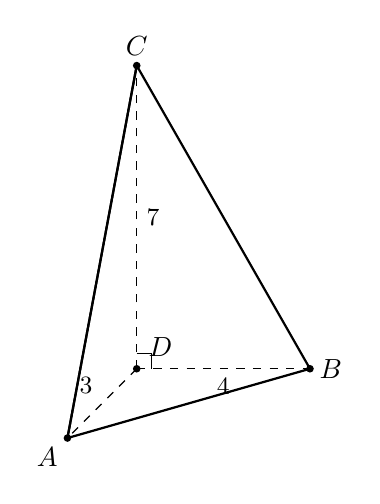
\begin{tikzpicture}[scale=0.55]
\coordinate (D) at (0,0); \coordinate (A) at (-1.6,-1.6); \coordinate (B) at (4,0); \coordinate (C) at (0,7);
\draw[thick] (A)--(B)--(C)--cycle; \draw[thick] (A)--(C); \draw[dashed] (D)--(A); \draw[dashed] (D)--(B); \draw[dashed] (D)--(C);
\draw (0,0.35)--(0.35,0.35)--(0.35,0);
\foreach \p in {A,B,C,D} \fill (\p) circle (2.5pt);
\node[below left] at (A){$A$}; \node[right] at (B){$B$}; \node[above] at (C){$C$}; \node[above right] at (0.05,0.05){$D$};
\node[above left] at (-0.8,-0.8){\small$3$}; \node[below] at (2,0){\small$4$}; \node[right] at (0,3.5){\small$7$};
\end{tikzpicture}}
$DA=3$, $DB=4$, $DC=7$ juft-jufti bilan perpendikulyar.

a) Yon yoqlar — töğri burçakli uçburçaklar:
\[S_{DAB}=\tfrac12\cdot3\cdot4=6,\quad S_{DBC}=\tfrac12\cdot4\cdot7=14,\quad S_{DAC}=\tfrac12\cdot3\cdot7=10{,}5.\]
Asos $ABC$ tomonlari: $AB^2=9+16=25$, \ $BC^2=16+49=65$, \ $AC^2=9+49=58$. Geron formulasining kvadratlar orqali körinişi:
\[16S^2=2(25\cdot65+65\cdot58+58\cdot25)-(25^2+65^2+58^2)=13690-8214=5476\ \Rightarrow\ S_{ABC}=\frac{74}4=18{,}5.\]
\[S_{\text{töla}}=6+14+10{,}5+18{,}5=49.\]
b) $V=\dfrac13\cdot S_{DAB}\cdot DC=\dfrac13\cdot6\cdot7=14$. Içki çizilgan şar radiusi:
\[r=\frac{3V}{S_{\text{töla}}}=\frac{42}{49}=\frac67.\]
\Javob{a) 49; \quad b) $\frac67$}

%================= 45
\newpage
\Savol{45}
\fig{\begin{tikzpicture}[scale=0.3]
\draw[->] (-4.5,0)--(4.8,0) node[right]{$x$}; \draw[->] (0,-0.5)--(0,10) node[above]{$y$};
\draw[thick,domain=-3:3,samples=60] plot (\x,{\x*\x});
\draw[thick] (-3,9)--(3,9);
\draw[thick,fill=msblue!20] (0,4.25) circle (2);
\draw[axs] (0,4.25)--(1.936,3.75); \draw[ax] (0,0)--(0,2.25);
\fill (0,4.25) circle (3pt); \fill[aux] (1.936,3.75) circle (3pt);
\node[aux,left] at (0,1.1){\small$2{,}25$}; \node[aux,above] at (1.0,4.05){\scriptsize$R$};
\node[right] at (3,9){\small$(3;9)$}; \node[left] at (-0.1,4.6){\scriptsize$Q$};
\end{tikzpicture}}
Öq kesimi: qadah tubini koordinata boşiga qöysak, uning devori — $y=kx^2$ parabola; $(3;9)$ nuqtadan ötadi: $k=1$, \ $y=x^2$.

a) Aylanma paraboloid hajmi — $y$ böyiça kesimlar doira, radiusi $x^2=y$:
$V=\pi\displaystyle\int_0^9y\,dy=\pi\cdot\frac{81}2=\frac{81\pi}2.$

b) Şar markazi $Q(0;\,2{,}25+R)$, radiusi $R$. Şar devorga urinadi: $Q$ dan parabola nuqtalarigaça eng kiçik masofa $R$ ga teng. $(x;x^2)$ nuqtagaça masofa kvadrati ($u=x^2$, $c=2{,}25+R$):
\[d^2=u+(u-c)^2,\qquad (d^2)'_u=1+2(u-c)=0\Rightarrow u=c-\tfrac12,\qquad d^2_{\min}=c-\tfrac14.\]
\[R^2=2{,}25+R-0{,}25\ \Rightarrow\ R^2-R-2=0\ \Rightarrow\ R=2\quad(u=3{,}75<9\ \text{— qadah içida}),\qquad V_{\text{konfet}}=\frac43\pi\cdot2^3=\frac{32\pi}3.\]
\Javob{a) $\frac{81\pi}2$; \quad b) $\frac{32\pi}3$}

\ShowJavoblar
\end{document}
